\documentclass[12pt,oneside]{report}

\usepackage[utf8]{inputenc}		% suport pentru diacritice
\usepackage{array}
\usepackage{booktabs}
\usepackage{graphicx}
\usepackage{float}
\usepackage{listings, xcolor}	% pentru a da ca exemplu json-uri
\usepackage{afterpage}			% pentru a adauga o pagina goala

\newcommand\blankpage{   
	\null
	\thispagestyle{empty}
	\addtocounter{page}{-1}
	\newpage}

\newlength\tindent
\setlength{\tindent}{\parindent}
\setlength{\parindent}{0pt}
\renewcommand{\indent}{\hspace*{\tindent}}
\setlength{\parskip}{0.6em}

\definecolor{background}{HTML}{EEEEEE}

\lstset{
	string=[s]{"}{"},
	stringstyle=\color{blue},
	comment=[l]{:},
	commentstyle=\color{black},
	backgroundcolor=\color{background}
}								% cum arata json-urilor date ca exemplu

\renewcommand{\contentsname}{Cuprins}
\renewcommand{\figurename}{Figura}
\renewcommand{\tablename}{Tabelul}
\renewcommand{\bibname}{Bibliografie}

% pentru ca numerotarea sectiunilor din capitole sa nu fie precedate de indexul capitolelor
\renewcommand{\thesection}{\arabic{section}}

\begin{document}

% Coperta lucrării de licenţă
\begin{center}
	\large{UNIVERSITATEA \ghilimele{ALEXANDRU IOAN CUZA} DIN IAȘI} \\
	\vspace{0.4cm}
	
	\large{\textbf{FACULTATEA DE INFORMATICĂ}} \\
	\vspace{1cm}
	
	
\includegraphics[
		width=2cm,
		height=3cm,
		keepaspectratio
	]
	{imagini/sigla_fii.png}\\
	\vspace{1cm}
	
	\large{\textbf{LUCRARE DE LICENȚĂ}}\\
	\vspace{1cm}
	
	\LARGE{Problema iterată a prizonierului. Calitatea soluțiilor oferite de un algoritm genetic în contextul turneelor eliminatorii} \\
	\vspace{1.4cm}
	
	\large\textbf{{propusă de}}\\ 
	\vspace{0.4cm}
	
	\large{\textbf{\textit{Denise-Mihaela Goldan}}}\\
	\vspace{2cm}
	
	\large{\textbf{Sesiunea:} Iulie, 2018}\\
	\vspace{2cm}
	
	\large{\textbf{Coordonator științific}}\\
	\vspace{0.4cm}
	
	\large{\textbf{Conf. dr. Adrian Iftene}}
\end{center}

%\afterpage{\null\newpage}

% Prima pagină a lucrării de licenţă
\begin{center}
	\large{UNIVERSITATEA \ghilimele{ALEXANDRU IOAN CUZA} DIN IAȘI} \\
	\vspace{0.4cm}
	
	\large{\textbf{FACULTATEA DE INFORMATICĂ}} \\
    \vspace{4cm}
    
	\LARGE{Problema iterată a prizonierului. Calitatea soluțiilor oferite de un algoritm genetic în contextul turneelor eliminatorii} \\
	\vspace{3cm}
	
	\large{\textbf{\textit{Denise-Mihaela Goldan}}}\\
	\vspace{2.5cm}
	
	\large{\textbf{Sesiunea:} Iulie, 2018}\\
	\vspace{2.5cm}
	
	\large{\textbf{Coordonator științific}}\\
	\vspace{0.4cm}
	
	\large{\textbf{Conf. dr. Adrian Iftene}}
\end{center}

\clearpage

%\afterpage{\null\newpage}

% Declaraţie standard privind originalitatea lucrării de licență
\begin{center}
	\textbf{\large{Declarație privind originalitatea \\conținutului lucrării de licență}}
\end{center}
	
\begin{flushright}
	Avizat,\\
	Îndrumător Lucrare de Licență\\
	Conf. dr. Adrian Iftene\\
	Data \small{..........................} Semnătura \small{...............................}
\end{flushright}

Subsemnata Goldan Denise-Mihaela, domiciliul in Strada Petru  Șchiopul nr.1, bloc L1A, scara A, etaj 1, apartament 3, născută la data de 27.09.1996, identificată prin CNP 2960927226702, absolventă a Universității \ghilimele{Alexandru Ioan Cuza} din Iași, Facultatea de Informatică, promoția 2015-2018, declar pe propria răspundere, cunoscând consecințele falsului în declarații în sensul art. 326 din Noul Cod Penal și dispozițiile Legii Educației Naționale nr. 1/2011 art.143 al. 4 si 5 referitoare la plagiat, că lucrarea de licență cu titlul \ghilimele{\textit{Problema iterată a prizonierului. Calitatea soluțiilor oferite de un algoritm genetic în contextul turneelor eliminatorii}} elaborată sub îndrumarea dl. Conf. dr. Adrian Iftene, pe care urmează să o susțină în fața comisiei este originală, îmi aparține și îmi asum conținutul său în întregime.

De asemenea, declar că sunt de acord ca lucrarea mea de licență să fie verificată prin orice modalitate legală pentru confirmarea originalității, consimțind inclusiv la introducerea conținutului său într-o bază de date în acest scop.

Am luat la cunoștință despre faptul că este interzisă comercializarea de lucrări științifice în vederea facilitării fasificării de către cumpărător a calității de autor al unei lucrări de licență, de diplomă sau de disertație și în acest sens, declar pe proprie răspundere că lucrarea de față nu a fost copiată ci reprezintă rodul cercetării pe care am întreprins-o.

\hfill \break

Dată azi, \small{..........................} \hfill Semnătură student \small{...............................} \\

\clearpage


% Declaraţie standard privind drepturile de utilizare a lucrării şi codului sursă
\hfill \break
\hfill \break

\begin{center}
	\textbf{\large{Declarație de consimțământ}}
\end{center}

\hfill \break
\hfill \break

Prin prezenta declar că sunt de acord ca Lucrarea de licență cu titlul \ghilimele{\textit{Problema iterată a prizonierului. Calitatea soluțiilor oferite de un algoritm genetic în contextul turneelor eliminatorii}}, codul sursă al programelor și celelalte conținuturi  (grafice, multimedia, date de test etc.) care însoțesc această lucrare să fie utilizate în cadrul Facultății de Informatică. 

De asemenea, sunt de acord ca Facultatea de Informatică de la Universitatea Alexandru Ioan Cuza Iași să utilizeze, modifice, reproducă și să distribuie în scopuri necomerciale programele-calculator, format executabil și sursă, realizate de mine în cadrul prezentei lucrări de licență. 

\hfill \break
\hfill \break
\hfill \break
\hfill \break

Iaşi, 29 Iunie 2018 \hfill Absolvent Denise-Mihaela Goldan\\

\clearpage

% Capitole 
\tableofcontents

% Problema iterata a prizonierului
\setcounter{section}{0}
\chapter*{Problema iterată a prizonierului}
\addcontentsline{toc}{chapter}{Problema iterată a prizonierului}
\section{Enunţul clasic al dilemei prizonierului}

Dilema prizonierului \cite{prisoner_s_dilemma_game_theory} reprezintă o problemă tratată în teoria jocurilor.

A fost formulată în anul 1950 de către Merrill Flood și Melvin Dresher, angajați ai companiei RAND Corporation \cite{rand_org}. Denumirea (dilema prizonierului) este meritul lui Albert W. Tucker, de la Universitatea Princeton, care a formalizat jocul și a introdus noțiunea de \textbf{răsplată} (engl. payoff).
 
Enunțul clasic al problemei este prezentat în paragraful următor: 

\begin{quote} 
	\textit{Doi suspecți sunt arestați de către poliție. Polițiștii nu au suficiente dovezi pentru a condamna suspecții, așa că îi duc în camere separate și le propun amândurora aceeași ofertă. Dacă unul dintre suspecți depune mărturie pentru urmărirea penală împotriva celuilalt suspect și celălalt tăinuiește faptele, cel care a trădat este eliberat și cel care a tăinuit primește o pedeapsă de 10 ani de închisoare. Dacă niciunul nu mărturiseşte, ambii ajung în pușcarie pentru jumătate de an. Dacă se trădează reciproc, fiecare primește o pedeapsă de 5 ani. Suspecții au de ales între a trăda și a tăinui faptele.}
\end{quote}


\begin{figure}[H]
	\centering
	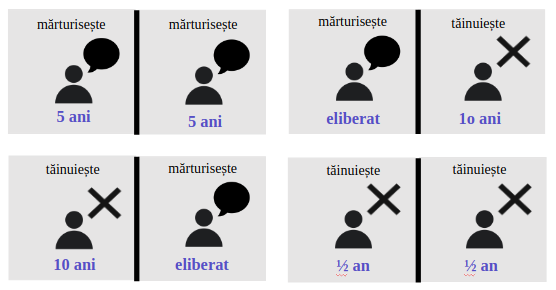
\includegraphics[
		width=15cm,
		height=8cm,
		keepaspectratio
	]{imagini/matrice.png}\\
	\caption{\textit{Prezentare a celor patru posibilități descrise în scenariul anterior.}}
	\label{fig:matrice_prezentare_scenarii}
\end{figure}

Observaţie: \textit{Considerăm că atunci când un suspect mărturisește, mărturia să îl incriminează pe celălalt suspect. Tăinuirea faptelor reprezintă decizia suspectului de a nu spune nimic anchetatorilor.}

Putem formaliza aceast paragraf prin următorul tabel al recompenselor, unde cei doi suspecți sunt numiți \textbf{A} și \textbf{B} \cite{plato_stanford}. Se prezintă rezultatele obținute pentru fiecare combinație dintre tăinuire și marturisire:  

\begin{table}[H]
	\centering
	\def\arraystretch{1.75}
	\begin{tabular}{|c|c|c|c|}
		\hline
		\multicolumn{2}{|c|}{\textbf{Acţiune aleasă}} & \multicolumn{2}{c|}{\textbf{Rezultat obţinut}} \\ \hline
		\textbf{A} & \textbf{B} & \textbf{A} & \textbf{B} \\ \hline
		tăinuiește & tăinuiește & \textbf{Reward} & \textbf{Reward} \\ \hline
		tăinuiește & mărturiseşte & \textbf{Sucker's payoff} & \textbf{Temptation} \\ \hline
		mărturiseşte & tăinuiește & \textbf{Temptation} & \textbf{Sucker's payoff} \\ \hline
		mărturiseşte & mărturiseşte & \textbf{Punishment} & \textbf{Punishment} \\ \hline
	\end{tabular}
	\caption{\textit{Adaptare după matricea recompenselor pentru dilema prizonierului}}
	\label{matricea_recompenselor}
\end{table}

Termenii care apar în tabel sunt următorii: 
 
\begin{itemize} 
	\item \textbf{Temptation}: recompensa obținută de jucatorul ce mărturisește atunci când celalalt tăinuiește faptele 
	\item \textbf{Reward}: recompensa pentru când cei doi suspecți, A și B, aleg să tăinuiască 
	\item \textbf{Punishment}: pedeapsa obținută de fiecare dintre cei doi suspecți atunci când se trădează reciproc 
	\item \textbf{Sucker's payoff}: pedeapsa pentru cel care a tăinuit atunci când celălalt l-a trădat 
\end{itemize} 
 
Pentru a face trecerea de la pedeapsa cu închisoarea la ideea de joc, considerăm că cei 4 termeni reprezintă scoruri de valoare pozitivă și că scopul suspecților este să obțină un număr cât mai mare de puncte. 

Între acești termeni ce reprezintă recompensele, se respectă următorul lanț de inegalități: 

\begin{center} 
	\textbf{Temptation} \textgreater \textbf{Reward} \textgreater \textbf{Punishment} \textgreater \textbf{Sucker's payoff} 
\end{center} 

\subsection{Strategii pentru dilema prizonierului}

Dacă suspectăm că celălalt reținut va tăinui faptele, suntem mai avantajați dacă mărturisim (vom fi "răsplătiți" cu \textbf{Temptation}, despre care știm că are o valoare mai mare decât \textbf{Sucker's payoff}- scorul pe care îl va obține celălalt suspect), decât dacă tainuim (caz în care toți primesc \textbf{Reward}; \textbf{Temptation} \textgreater \textbf{Reward}).

Dacă suspectăm că celălalt va mărturisi împotriva noastră, suntem mai avantajați dacă mărturisim și noi (vom primi amândoi \textbf{Punishment}), decât dacă tainuim (caz în care primim \textbf{Sucker's payoff}, însă celalt va primi un scor mai bun, \textbf{Temptation}).

În alte cuvinte, indiferent de mișcarea celuilalt jucător, \textit{strategia care ne avantajează câștigul personal, în defavoarea câștigului celuilalt jucător, este mărturisirea împotriva acestuia}.

Dilema este dată de faptul că ambii suspecți ar fi obținut un scor mult mai bun dacă ar fi tăinuit amândoi (protejând pe celălalt participant), decât dacă amândoi ar fi ales să mărturisească (în defavoarea celuilalt suspect). Pe scurt, \textit{cooperarea celor doi aduce cel mai mare avantaj de ambele părți}.

\section {Varianta iterată a dilemei prizonierului} 

Dacă s-ar juca mai multe runde, în care ambii jucători ar alege să se trădeze reciproc la fiecare rundă, scorul pe care l-ar obține ar fi mult mai mic decât dacă ar alege să tainuiasca faptele în fiecare rundă. 

În teoria jocurilor, problema iterată a prizonierului este catalogată drept joc cu suma nenulă \footnote{Numim joc de sumă nenulă jocul în care suma câstigurilor este diferită de zero.} (engl. non-zero-sum game).

Un meci între doi jucători este reprezentat de un număr de runde, care nu este cunoscut de catre participanți.

În fiecare rundă, cei doi jucatarori aleg independent, în secret, ce mișcare vor face: vor tăinui sau vor mărturisi. La final de rundă, cei doi își expun alegerea. În funcție de ce mișcare au ales cei doi, fiecare este răsplătit cu un anumit câștig, care se adaugă la scorul total individual al jucătorilor. 

Dacă la o anumită rundă ambii au cooperat, scorul ambilor jucători va crește cu o valoare ce poartă denumirea de \textbf{Reward}. 

Dacă ambii trădează, vor primi \textbf{Punishment payoff}. 

Dacă unul cooperează, dar celălalt trădează, cel care a cooperat primește \textbf{Sucker's payoff} și celălalt este răsplătit cu \textbf{Temptation}. 

\subsection {Strategii pentru problema iterată a prizonierului}

Considerând acest scenariu drept un joc, folosim termenul de \textbf{cooperare} (engl. cooperation) pentru a descrie situația când unul dintre suspecți \textbf{tăinuiește} faptele. \textbf{Mărturisirea} faptelor de către un suspect pentru incriminarea celuilalt suspect va fi numită \textbf{trădare} (engl. defection). 

\subsubsection{Turneele lui Axelrod}

Printre studiile pofesorului Robert Axelrod, care predă științe politice și politici publice la Universitatea din Michigan, se află și problema iterată a prizonierului.

Interesul său de a afla o strategie potrivită l-a determinat să organizeze două turnee de tip \textit{fiecare cu fiecare} (engl. round-robin). În aceste turnee, fiecare participant joacă pe rând împotriva tuturor celorlalți \cite{round_robin_dictionary}. Primul turneu a inclus 14 programe ce furnizează strategii de joc, iar cel de al doilea a avut un număr de 63 de programe. Observațiile sale sunt trecute în lucrarea \textit{The Evolution of Cooperation}, scrisă în 1984 \cite{article_by_melanie_mitchell}. Axelrod a solicitat participanților strategii sub formă unor programe care cunosc istoricul ultimelor trei runde.

Câștigătorul ambelor turnee a fost strategia \textbf{Tit-for-Tat}. Această strategie cooperează la prima rundă, apoi, în următoarele runde, utilizează mișcarea făcută de oponent în runda anterioară. În alte formă de idei, cooperează de fiecare dată când celălalt cooperează și trădează când este trădată, dar nu inițiază trădarea.

\clearpage

\subsubsection{Strategii analizate}

În următoarele rânduri, sunt enumerate câteva strategii analizate:

\begin{itemize}  
	\item \textbf{Always cooperate}: Jucătorul cooperează la fiecare rundă a jocului, indiferent de strategia aplicată de celălalt jucător. 
	\item \textbf{Always defect}: Jucătorul trădează la fiecare rundă a jocului. 
	\item \textbf{Grudger}: Această strategie presupune cooperarea la fiecare rundă, până la prima trădare din partea celuilalt jucător. Așadar, adoptând această strategie, dacă oponentul trădează chiar și o singură dată, următoarele mișcări, până la final de joc, vor fi de trădare. 
	\item \textbf{Pavlov}: Se alege cooperarea la prima rundă. Dacă la runda anterioară jucătorul a fost recompensat cu \textbf{Temptation}\footnote{\textbf{Temptation} este recompensa obținută de jucatorul ce trădează atunci când oponentul cooperează.} sau \textbf{Reward}\footnote{\textbf{Reward} reprezintă recompensa primită de ambii jucători atunci când cooperează.}, acesta repetă ultima mișcare. În celălalt caz, alege mișcarea opusă. 
	\item \textbf{Random}: Se alege la întâmplare următoarea acțiune. 
	\item \textbf{Tit-For-Tat}: Se alege cooperarea la prima rundă. De la runda a doua, jocuatorul ce alege această strategie repetă ultima mișcare a oponentului. 
	\item \textbf{Suspicious Tit-For-Tat}: Diferența dintre această strategie și \textbf{Tit-For-Tat} este că la prima mișcare se alege trădarea. 
	\item \textbf{Tit-For-Two-Tats}:  Jucătorul cooperează de fiecare dată, făcând excepție acele cazuri în care jucătorul este trădat de două ori consecutiv. 
\end{itemize}  




% Algoritm genetic
\setcounter{section}{0}
\chapter*{Algoritm genetic}
\addcontentsline{toc}{chapter}{Algoritm genetic}
\section{ Aparitia notiunii de algoritm genetic }

\begin{center}
	\textit{Computer programs that "evolve" in ways that resemble natural selection can solve complex problems even their creators do not fully understand. }
\end{center}
by John H. Holland 

Propusi de John Holland, profesor la Universitatea din Michigan.

Algoritmii genetici au fost creati in incercarea de a imita procese specifice evolutiei naturale, cum ar fi lupta pentru supravietuire si mostenirea materialului genetic. Putem privi evolutia drept strategia abordata de speciile biologice pentru a cauta "solutii" cat mai potrivite, adaptate conditiilor schimbatoare, intr-un numar foarte mare de posibilitati. Aceasta abordare poate fi utilizata in rezolvarea problemelor de optimizare, atunci cand metodele clasice exhaustive nu se dovedesc eficiente.

\cite{introduction_by_melanie_mitchell}
Notiunea de "algoritm genetic" nu este definita in mod riguros, insa toate metodele ce poarta aceasta denumire au in comun urmatoarele: populatia este formata din cromozomi, selectiz este facuta pe baza rezultatelor functiei de optimizat, incrucisarea a doi \textit{cromozomi parinti} produce 2 \textit{cromozomi copii}, mutatia se aplica \textit{cromozomilor copii}\cite{introduction_by_melanie_mitchell}.

\section{Terminologie de specialitate}

\begin{itemize}
	
	\item Solutiile candidat sunt adesea codificate in forma unor siruri de biti si se mai numesc \textbf{cromozomi} sau \textbf{indivizi} ai populatiei. Fiecare bit este echivalentul unei gene.
	
	\item Genele sunt informatiile stocate de catre cromozomi.
	
	\item \textbf{Populatia}, care va fi urmarita in procesul sau evolutiv, este alcatuita din mai multi cromozomi.
	
	\item Fiecare \textbf{generatie} marcheaza cate o etapa din evolutia populatiei initiale.
	
	\item Pentru a trece de la o generatie la alta, apelam la notiunea de \textbf{reproducere}. In alcatuirea urmatoarei generatii, se porneste de la populatia actuala, pe care o supunem unui proces de \textbf{selectie}. Pentru a face analogia cu fenomenul de supravietuire a celor mai adapati indivizi, masuram cromozomii cu ajutorul unei functii de optimizat. O valoare ridicata a acestei functii este interpretata ca o buna adaptare la mediu a individului. 
	
	\item Pentru explorarea spatiului de solutii, indivizii selectati sufera modificari. Sunt supusi \textbf{incrucisarilor} si \textbf{mutatiilor}.
	
\end{itemize}

Operatori genetici

Mutatia 

Incrucisarea

Explorare si exploatare

Cautarea solutiei optimale apeleaza la doua mecanisme, denumite explorare si exploatare. 
Explorarea inseamna tendinta de a cauta solutii noi in spatiul e solutii. Pentru asta apelam la operatorii genetici. Exploatarea inseamna rafinarea solutiilor obtinute in urma explorarii, pentru care solosim diverse tehnici de selectie.


Algoritmul modifica in mod repetat populatia de solutii candidat. Se urmareste ca populatia sa evolueze catre obtinerea solutiiei optimale.

Over successive generations, the population "evolves" toward an optimal solution.

Procesul de evolutie este simulat iterand printr-o succesiune de generatii, unde, aplicand criteriu de selectie asupra opulatiei curente, se obtine viitoarea generatie. Criteriul de selectie este astfel formulat incat sunt favorizati acei candidati care au rezultate mai bune ale functiei de optimizat, deoarece indivizii care se adapteaza cel mai bine mediului au sanse mai mari de supravietuire. Asupra acestei poulatii selectate se aplica operatori genetici, mutatia si incrucisarea.
Populatia




evolutia este simulata printr-o succesiune de generatii ale unei populatii de solutii candidat;
o solutie candidat poarta numele de cromozom si este reprezentata ca un sir de gene;
gena este informatia atomica dintr-un cromozom;
pozitia pe care o ocupa o gena se numeste locus;
toate valorile posibile pentru o gena formeaza setul de alele ale genei;
populatia evolueaza prin aplicarea operatorilor genetici: mutatia si incrucisarea;
cromozomul asupra caruia se aplica un operator genetic se numeste parinte iar cromozomul rezultat se numeste descendent;
selectia este procedura prin care sunt alesi cromozomii ce vor supravietui in generatia urmatoare; indivizilor mai bine adaptati li se vor da sanse mai mari;
gradul de adaptare la mediu este masurat de functia de optimizat;
solutia returnata de un algoritm genetic este cel mai bun individ din ultima generatie.


Pseudocod

initializeaza cu valori aleatorii populatia initiala
calculeaza valoarea functiei de optimizat pentru indivizii populatiei 
cat timp nu s-a indeplinit conditia de oprire
	aplica o metoda de selectie, pentru a crea populatia
	aplica operatorul genetic incrucisare, cu o anumita probabilitate
	aplica operatorul genetic mulatie, cu o anumita probabilitate
	calculeaza valoarea functiei de optimizat pentru indivizii populatiei
	
Conditia de oprire poate fi atingerea unui numar de iteratii stabilit initial. De asemenea, se poate stabili ca algoritmul sa se opreasca atunci cand nu se mai inregistreaza imbunatatiri in ceea ce priveste calitatea solutiilor furnizate. 


solutia returnata de un algoritm genetic este cel mai bun individ din ultima generatie 

- cum se face un asemenea algoritm pentru aceasta problema?
- care sunt limitarile unui algoritm genetic aplicat pe acasta problema?

Prin utilizarea unui algoritm genetic, pot obtine o copie a celui mai bun individ din toate generatiile care au participat la antrenare. In alte cuvinte, acest cromozom contine strategia care a obtinut cel mai bun scor. Pentru crearea acestui individ, este nevoie de ajustarea mai multor parametri si optiuni, dintre care mentionez: rata mutatiei, rata incrucisarii, tipul selectiei populatiei (populatia difera usor de la generatie la generatie, selectandu-se doar anumiti indivizi si in anumite proportii). Cromozomul are capacitatea de a-si formula urmatoarea miscare bazandu-se pe istoricul ultimelor 3 runde. Din acest motiv este important ca un meci sa fie format din mai multe runde. Asadar, numarul de runde reprezinta si acesta un parametru pentru antrenarea cromozomilor. 


\hfill \break
\hfill \break

\clearpage

% Dezvoltarea unei strategii folosind un algoritm genetic
\setcounter{section}{0}
\chapter*{Dezvoltarea unei strategii pentru problema iterată a prizonierului folosind un algoritm genetic}
\addcontentsline{toc}{chapter}{Dezvoltarea unei strategii pentru problema iterată a prizonierului folosind un algoritm genetic}
\section{Modelarea unui algoritm genetic pentru problema iterată a prizonierului}

\subsection{Reprezentarea soluției}

În urma organizării celor două turnee, Axelrod a decis să cerceteze dezvoltarea unei strategii pentru problema iterata a prizonierului, folosindu-se de algoritmii genetici introduși de Holland. 

Unul din cei mai importanți pași din acest proces a fost stabilirea unei modalități de a reprezenta o strategie în forma unui cromozom. Descriem concluziile lui Axelrod în rândurile următoare.

Presupunem că fiecare jucător are capacitatea de a memora mișcările ultimei runde sub forma unei perechi- primul element reprezintă mișcarea proprie, iar cel de al doilea element reprezintă mișcarea oponentului. Ne vom folosi de următoarea notație:

\begin{center}
	\textbf{C} reprezintă \textbf{cooperarea cu oponentul}\\
	\textbf{T} reprezintă \textbf{trădarea oponentului}   
\end{center}

Există patru perechi (sau cazuri) posibile:\\

\begin{center}
	Cazul 1: \textbf{CC}\\
	Cazul 2: \textbf{CT}\\
	Cazul 3: \textbf{TC}\\
	Cazul 4: \textbf{TT}\\
\end{center}

Pentru acest scenariu, strategia reprezintă ce mișcare vom alege, dat fiind aflarea mișcării oponentului în ultima rundă.

Strategia \textbf{Tit-for-Tat} este reprezentată în felul următor: 

\begin{center}
	dacă \textbf{CC} atunci \textbf{C}\\
	dacă \textbf{CT} atunci \textbf{T}\\
	dacă \textbf{TC} atunci \textbf{C}\\
	dacă \textbf{TT} atunci \textbf{T}\\
\end{center}

Dacă impunem ca aceste patru cazuri să respecte ordinea lexicografică, putem codifica strategia drept șirul de caractere \textbf{CTCT}. Ca să utilizăm această reprezentare a strategiei:\\
\begin{itemize}
	\item Observăm ce a ales oponentul în runda anterioară;
	\item Formăm perechea compusă din mișcarea noastră, împreună cu cea a oponentului;
	\item Vedem indexul care corespunde perechii obținute la pasul anterior;
	\item Alegem mișcarea pe care o găsim la indexul respectiv.
\end{itemize}

Strategiile lui Axelrod se bazau pe istoricul ultimelor trei runde. Pentru acestea, există 64 \footnote{64, sau $2^6$, reprezintă numărul de șiruri de caractere unice pe care le putem genera folosind doar caracterele \textbf{C} și \textbf{T}} de posibile scenarii pentru utlimele trei runde: 

\begin{center}
	Cazul 1: \textbf{CC CC CC}\\
	Cazul 2: \textbf{CC CC CT}\\
	Cazul 3: \textbf{CC CC TC}\\
	...
	\\
	Cazul 62: \textbf{TT TT CT}\\
	Cazul 63: \textbf{TT TT TC}\\
	Cazul 64: \textbf{TT TT TT}\\
\end{center}

Ca și în  ipoteza în care jucătorii memorează doar istoricul ultimei runde, putem reprezenta aceste cazuri într-un șir de caractere de lungime 64. Vom folosi un șir de caractere de lungime 71, pentru a reține și ce mișcări ar trebui făcute în primele runde, când încă nu există un istoric care să cuprindă ultimele trei runde. Cele 7 poziții de la începutul șirului de caractere au următoarele semnificații:\\

\begin{enumerate}
	
	\item La \textbf{poziția numărul 1} se găsește mișcarea aleasă pentru prima rundă a jocului;
	
	\item \textbf{Poziția numărul 2}: mișcarea pentru cea de a doua rundă, dacă la rundă anterioară oponentul a cooperat (\textbf{C} reprezintă istoricul mișcărilor oponentului);
	
	\item \textbf{Poziția numărul 3}: mișcarea pe care o vom face la cea de a două rundă, dacă la rundă anterioară oponentul a trădat (istoricul mișcărilor oponentului este scris sub forma \textbf{T});
	
	\item \textbf{Poziția numărul 4}: mișcarea pe care o vom face la cea de a două rundă, dacă pentru primele două runde, istoricul oponentului este \textbf{CC};
	
	\item \textbf{Poziția numărul 5}: mișcarea pentru cea de a treia rundă, dacă pentru primele două runde, istoricul oponentului este \textbf{CT};
	
	\item \textbf{Poziția numărul 6}: mișcarea pentru cea de a treia rundă, dacă pentru primele două runde, istoricul oponentului este \textbf{TC};
	
	\item \textbf{Poziția numărul 7}: mișcarea pentru cea de a treia rundă, dacă la primele două runde oponentul a avut mișcările \textbf{TT}.
	
\end{enumerate}

\subsection{Dimensiunea spațiului de căutare}

Având 71 de poziții pe care le putem ocupa cu cele două caractere- \textbf{C} sau \textbf{T}-, putem genera $2^{71}$ șiruri de caractere distincte. Acest număr reprezintă numărul tuturor strategiilor pe care îl putem avea, în contextul în care cunoaștem istoricul ultimelor trei runde ale jocului.  

Spațiul de căutare este, în concluzie, mult prea mare pentru a caută exhaustiv cea mai bună strategie.

\subsection{Funcția de optimizat}

Axelrod a alcătuit un set de opt strategii cu care să concureze fiecare strategie a algoritmului genetic, în vederea calculării unei funcții de optimizat. Acest set de strategii nu include strategia \textbf{Tit-for-Tat}. Valoarea funcției de optimizat este dată de media scorurilor obținute în urma meciurilor jucate cu fiecare dintre ele opt strategii.

\subsection {Parametrii algoritmului genetic}

Prin utilizarea unui algoritm genetic, pot obține o copie a celui mai bun individ din toate generațiile care au participat la antrenare. În alte cuvinte, acest cromozom conține strategia care a obținut cea mai bună valoare a funcției de optimizat. 

Pentru crearea acestui individ, este nevoie de ajustarea mai multor parametri și opțiuni, dintre care menționez: ratamutației, rata încrucisării, tipul selecției populației (populația diferă ușor de la generație la generație, selectandu-se doar anumiți indivizi și în anumite proporții). Cromozomul are capacitatea de a-și formulă următoarea mișcare bazându-se pe istoricul ultimelor trei runde. Din acest motiv este important ca un meci să fie format din mai multe runde. Așadar, numărul de runde reprezintă și acesta un parametru pentru antrenarea cromozomilor. 

-- OBSERVAȚII CLARE OBȚINUTE ÎN URMĂ UNOR EXPERIMENTE legat de modul în care parametrii influențează calitatea soluțiilor

\section {Elemente legate de implementarea algoritmului genetic}

-- CUM AM IMPLEMENTAT EU ACEASTĂ PROBLEMA

-- UȘURINȚA CU CARE SE POATE CREA O NOUĂ STRATEGIE

-- UNIT TESTS

\section {Limitările algoritmului genetic}

- care sunt limitările unui algoritm genetic aplicat pe această problema?

% Turnee
\setcounter{section}{0}
\chapter*{Turnee eliminatorii între strategii}
\addcontentsline{toc}{chapter}{Turnee eliminatorii între strategii}
Ne interesează să găsim \textit{cea mai bună strategie}. Pentru a compara între ele mai multe strategii, trebuie să gândim \textit{un mediu în care acestea să concureze}. 
 
Până la a găsi cea mai bună strategie, trebuie, mai întâi, să vedem cum anume poate configurația unui algoritm genetic să influențeze calitatea soluției. De asemenea, vrem să vedem cum anume se comportă într-un mediu de test strategia propusă de algoritm. 
 
Pentru a îndeplini aceste cerințe, am ales să supun cromozomii la un anumit tip de turneu, ce poartă denumirea de \textbf{turneu cu eliminare}.  

\section {Termeni întâlniţi}
O \textbf{rundă} este dată de alegerea, în mod secret, a mișcării următoare și actualizarea scorului în funcție de ce a pus și oponentul. 

Un \textbf{meci} este jucat de către doi jucători. Este alcătuit dintr-un număr de runde. În fiecare rundă, fiecare jucător alege, în mod secret, ce mișcare va face. La final de rundă, scorul jucătorilor este actualizat cu o valoare dată de mișcarea făcută de fiecare, în funcție de ce a ales și oponentul să facă. 

\section {Cum este modelat un turneu cu eliminare}
 
Un turneu cu eliminare pornește de la o populație de strategii în care, la fiecare iterație, fiecare individ joacă câte un meci cu ceilalți indivizi. Pe parcursul meciurilor, câștigurile individuale se însumează într-un scor total. După ce se joacă toate combinările de doi jucători (se ajunge la finalul iterației), se elimină un procent din cei mai slabi jucători.  Pentru a mai reduce din numărul parametrilor ale căror valori pot varia, am stabilit ca procentul să fie de 25\%. În caz de egalitate a scorurilor între doi jucători, se elimină la întâmplare unul din cei doi. Se completează locurile eliberate cu stategii care au obținut printre cele mai bune scoruri. Se resetează scorul total al indivizilor și se repetă acești pași până când în turneu a rămas un singur tip de strategie, ori până când am atins un număr maxim de iterații.  
\\\\
Observație: \textit{Când într-un turneu cu eliminare concurează doi indivizi ce au aceeași strategie deterministă, la finalul unei iterații, cei doi indivizi vor avea exact același scor. Nu putem spune același lucru despre doi indivizi care folosesc strategia \textbf{Random}.}
\\\\
Pentru a vedea clar modul în care evoluează strategiile în contextul acestui tip de turneu, am implementat o metodă grafică de vizualizare a datelor. Am ales să folosesc \textbf{line chart}-uri. Axa absciselor are drept legendă numărul de indivizi din fiecare strategie. Axa ordonatelor reprezintă numărul meciului din turneu.

\section{Configurația unui turneu cu eliminare}

Așa cum am stabilit parametrii mediului de antrenare (parametrii algoritmului genetic), va trebui să stabilim și în ce condiții vom testa cromozomii obținuți. Vom impune condiții legate de procentul de jucători care sunt eliminați, respectiv duplicați la final de iterație. De asemenea, vom stabili configurația populației de testare și câte copii după o anumită strategie a algoritmului genetic vor participa la turneul eliminatoriu. În ultimă instanță, vom alege numărul de runde ce va alcătui un meci dintre doi jucători. 
 
Cum s-a discutat în capitolul anterior, populația de testare va putea fi definită în fișierul \textbf{testing.config.json}.

În experimentele descrise, am ales ca participanții la turneu să aibă ponderi egale iar procentul de  jucători eliminați să fie de 25\%. 

\section {Concluzii trase în urma finalizării turneelor}

Fiecare experiment este dat de stabilirea parametrilor configurației algoritmului genetic, urmată de rularea algoritmului genetic și trecerea soluției prin mai multe medii de testare, prin varierea configurației turneului cu eliminare.

În contextul acestei probleme, nu putem vorbi despre optim local sau global, întrucât un fitness cu o valoare bună obținut pentru un cromozom în faza de antrenare poate să își piardă relevanța în faza de testare, datorită faptului că mediul de testare poate varia. 

În rândurile următoare prezint o serie de experimente.  

\subsection {Explorarea redusă a spațiului de căutare} 

\begin{center}
	\underline{\textit{Experimentul 1}}
\end{center}

\textit{Configurația algoritmului genetic și cea a turneului cu eliminare este trecută în \textbf{Anexa numărul 1}}.\\

Am făcut un prim experiment în care configurația algoritmului genetic a dus la o explorare redusă a spațiului de căutare. Pentru aceasta, am ales valori mici pentru numărul de generații (100), pentru numărul de runde din turneul clasic (10) și pentru probabilitățile operatorilor genetici (10\%).
 
Diagramele de mai jos atestă calitatea redusă a soluției obținute în urma rulării algoritmului genetic. 

\begin{figure}[H]
	\centering
	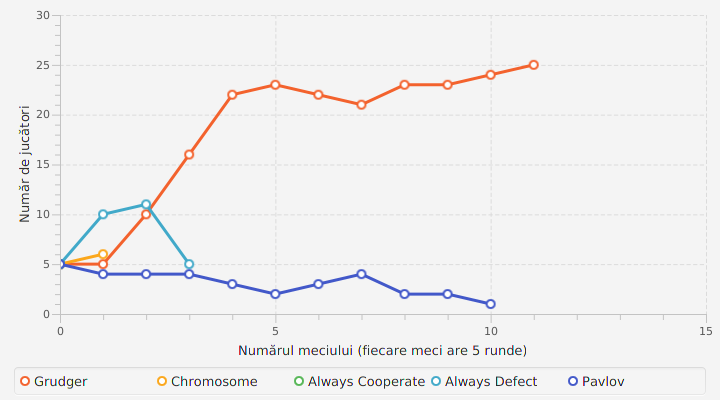
\includegraphics[	
	width=16cm,
	height=7.5cm,
	keepaspectratio
	]{imagini/experiment_1_epoch_1529303072346/chart_from_epoch_1529303304972.png}
	\caption{\textit{Cromozomii pierd în turneul cu eliminare cu 5 runde/meci.}}
\end{figure}

\begin{figure}[H]
	\centering
	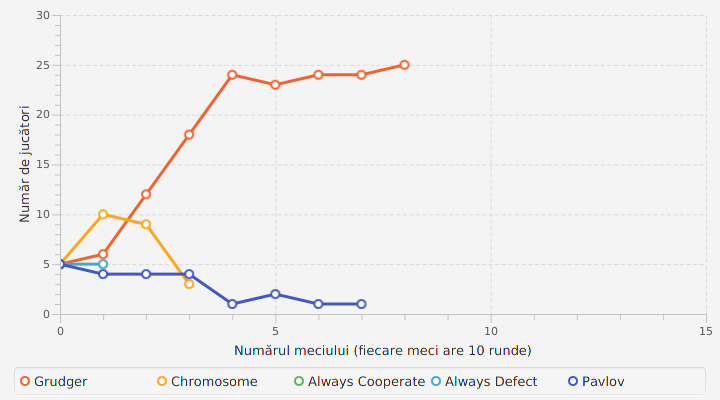
\includegraphics[	
	width=16cm,
	height=7.5cm,
	keepaspectratio
	]{imagini/experiment_1_epoch_1529303072346/chart_from_epoch_1529303340019.png}
	\caption{\textit{Cromozomii pierd în turneul cu eliminare cu 10 runde/meci.}}
\end{figure}

\begin{figure}[H]
	\centering
	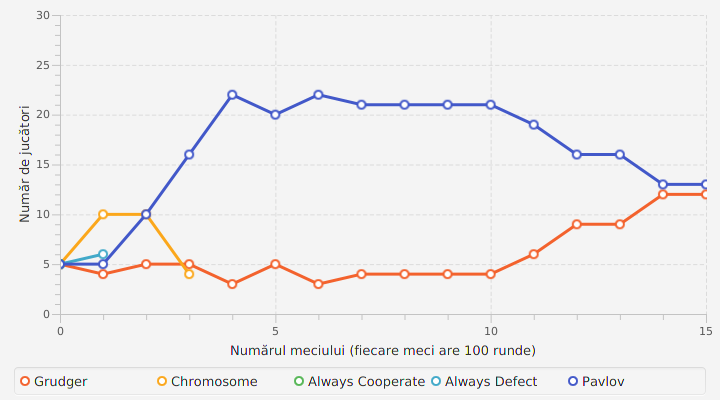
\includegraphics[	
	width=16cm,
	height=7.5cm,
	keepaspectratio
	]{imagini/experiment_1_epoch_1529303072346/chart_from_epoch_1529303352244.png}
	\caption{\textit{Cromozomii pierd în turneul cu eliminare cu 100 runde/meci.}}
\end{figure}

\begin{figure}[H]
	\centering
	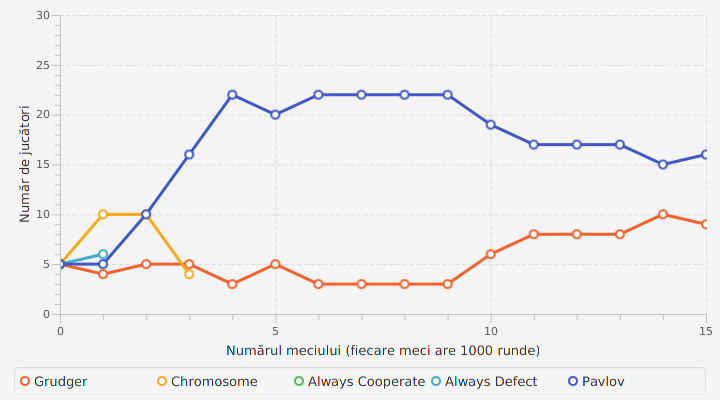
\includegraphics[	
	width=16cm,
	height=7.5cm,
	keepaspectratio
	]{imagini/experiment_1_epoch_1529303072346/chart_from_epoch_1529303371162.png}
	\caption{\textit{Cromozomii pierd în turneul cu eliminare cu 1000 runde/meci.}}
\end{figure}

\subsection {Numărul de runde al meciurilor din turneul cu eliminare}

\begin{center}
	\underline{\textit{Experimentul 2}}
\end{center}

\textit{Configurația algoritmului genetic și cea a turneului cu eliminare este trecută în \textbf{Anexa numărul 2}}.\\

Într-un alt experiment, am surpins cum numărul de runde al meciurilor din turneul cu eliminare, odată modificat cu o valoare foarte mică, a avantajat una din strategiile algoritmului genetic. 

\begin{figure}[H]
	\centering
	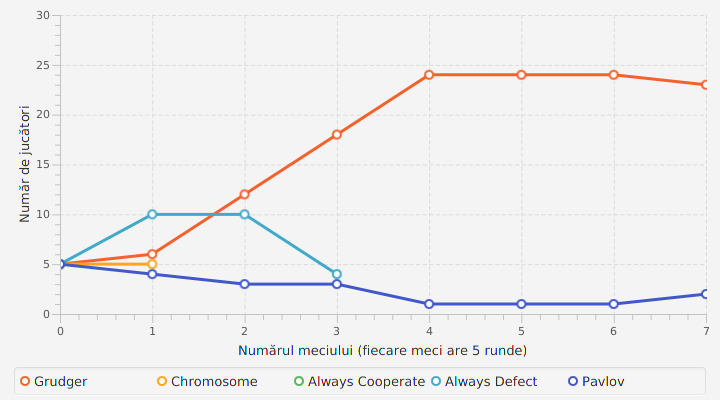
\includegraphics[	
	width=16cm,
	height=7.5cm,
	keepaspectratio
	]{imagini/experiment_2_epoch_1529309949939/chart_from_epoch_1529310422567.png}
	\caption{\textit{Cromozomii pierd în turneul cu eliminare cu 5 runde/meci.}}
\end{figure}

\begin{figure}[H]
	\centering
	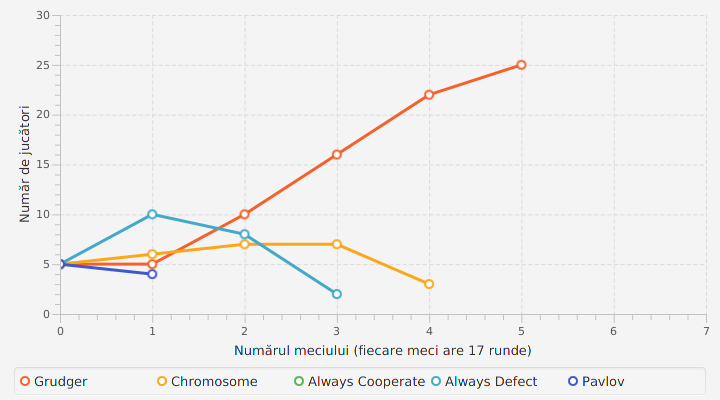
\includegraphics[	
		width=16cm,
		height=7.5cm,
		keepaspectratio
	]{imagini/experiment_2_epoch_1529309949939/chart_from_epoch_1529310399495.png}
	\caption{\textit{Cromozomii pierd în turneul cu eliminare cu 17 runde/meci.}}
\end{figure}

Mărind cu 1 numărul de runde din fiecare meci, observăm că strategia propusă de algoritmul genetic câștigă. 

\begin{figure}[H]
	\centering
	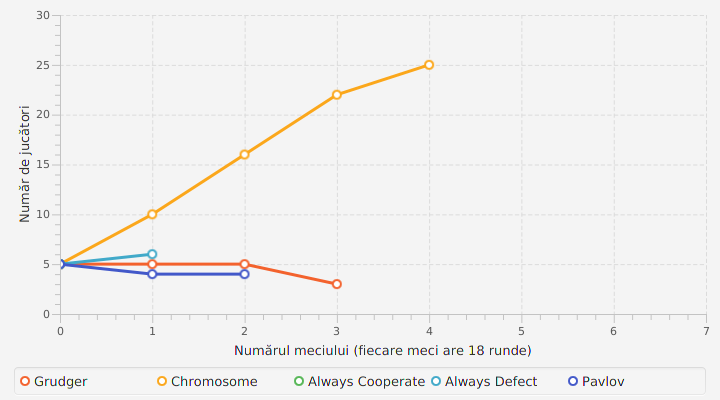
\includegraphics[	
	width=16cm,
	height=7.5cm,
	keepaspectratio
	]{imagini/experiment_2_epoch_1529309949939/chart_from_epoch_1529310386663.png}
	\caption{\textit{Cromozomii câștigă în turneul cu eliminare cu 18 runde/meci.}}
\end{figure}

\subsection{Strategia \textbf{Random}}

Strategia \textbf{Random} nu reprezintă o problemă pentru strategiile oferite de algoritmul genetic.

Am antrenat o populație de dimensiune mică (5 cromozomi) într-un număr mare de generații (1000), lansând valori mari ale mutației și încrucișării (50\% pentru ambii operatori). Populația de antrenament este dată de un singur individ de tip \textbf{Random}. Am rulat două experimente, în urma cărora am obținut două strategii: pentru prima strategie obținută, cea din experimentul numărul 3, numărul de runde al meciurilor tuneului clasic este mai mic (5 runde); pentru celălalt experiment numărul de runde al meciurilor din turneului clasic este 100.

\begin{center}
	\underline{\textit{Experimentul 3}}
\end{center}

\textit{Configurația algoritmului genetic și cea a turneului cu eliminare este trecută în \textbf{Anexa numărul 3}}.\\

\begin{figure}[H]
	\centering
	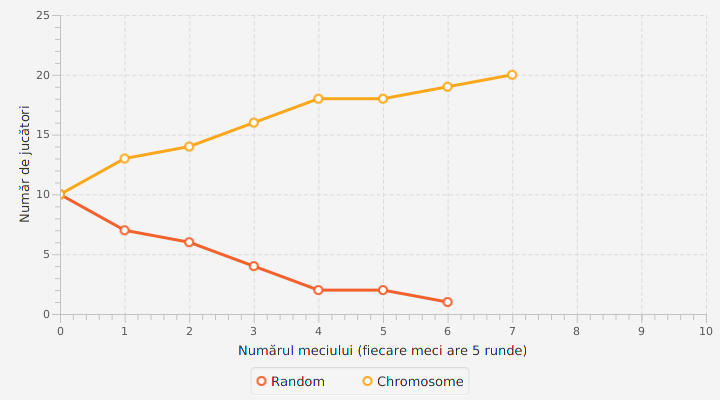
\includegraphics[	
	width=16cm,
	height=7.5cm,
	keepaspectratio
	]{imagini/experiment_3_epoch_1529321586156/chart_from_epoch_1529323404815.png}
	\caption{\textit{Cromozomii câștigă în turneul cu eliminare cu 5 runde/meci.}}
\end{figure}

\begin{figure}[H]
	\centering
	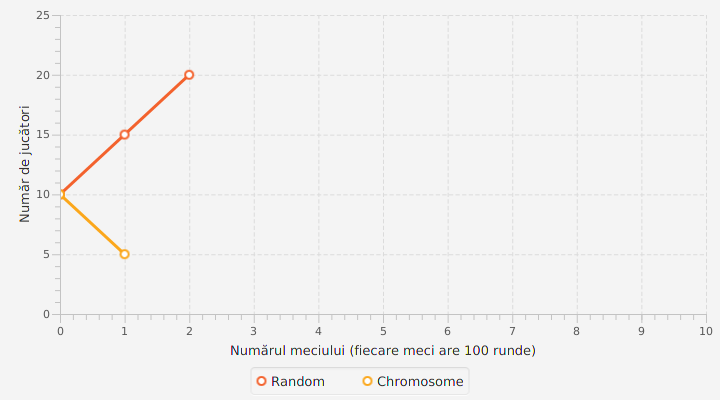
\includegraphics[	
	width=16cm,
	height=7.5cm,
	keepaspectratio
	]{imagini/experiment_3_epoch_1529321586156/chart_from_epoch_1529323424012.png}
	\caption{\textit{Strategia propusă de algoritmul genetic pierde, întrucât nu este optimizată pentru a câștiga în contextul unui turneu cu număr mare de runde.}}
	\label{pierde_cromozomul_castiga_random}
\end{figure}

\begin{center}
	\underline{\textit{Experimentul 4}}
\end{center}

\textit{Configurația algoritmului genetic și cea a turneului cu eliminare este trecută în \textbf{Anexa numărul 4}}.\\

\begin{figure}[H]
	\centering
	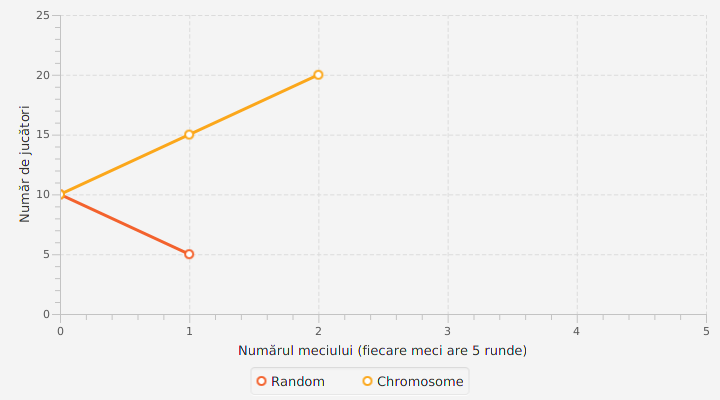
\includegraphics[	
	width=16cm,
	height=7.5cm,
	keepaspectratio
	]{imagini/experiment_4_epoch_1529323027289/chart_from_epoch_1529323309315.png}
	\caption{\textit{Cromozomii câștigă în turneul cu eliminare cu 5 runde/meci.}}
\end{figure}

\begin{figure}[H]
	\centering
	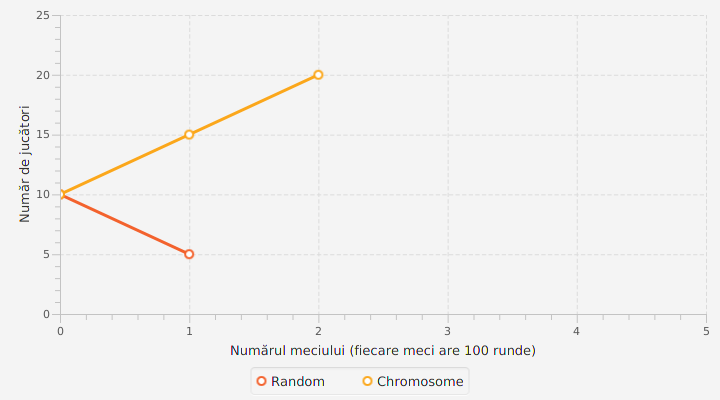
\includegraphics[	
	width=16cm,
	height=7.5cm,
	keepaspectratio
	]{imagini/experiment_4_epoch_1529323027289/chart_from_epoch_1529323321406.png}
	\caption{\textit{Cromozomii câștigă în turneul cu eliminare cu 100 runde/meci.}}
\end{figure}

Strategia din experimentul cu numărul 4 va face față și la un număr de runde mai mic, dar și la un număr de runde mai mare în turneele cu eliminare în fața strategiei \textbf{Random}. Pentru această configurație a turneului eliminatoriu, putem trage concluzia că experimentul numărul 4 oferă o soluție mai bună. 

\subsection{Strategia \textbf{Tit-For-Tat}}

\begin{center}
	\underline{\textit{Experimentul numărul 5}}
\end{center}

\textit{Configurația algoritmului genetic și cea a turneului cu eliminare este trecută în \textbf{Anexa numărul 5}}.\\

Un lucru ce se observă ușor este că strategia \textbf{Tit-For-Tat} reușește să câștige aproape de fiecare dată când la iniţializarea turneului cu eliminare toate strategiile au ponderi egale și numărul de runde/meci este mare.
 
Pentru a bate strategia \textbf{Tit-For-Tat} este necesar un număr mic de runde, fiindcă știm că un meci între doi astfel de indivizi le va crește substanțial scorul, întrucât cooperează la fiecare pas. De asemenea, trebuie să ne folosim de faptul că știm că va coopera la prima mișcare. Strategia inamică se va folosi de faptul că atunci când unul cooperează și celălalt trădează, cel care trădează este mai bine răsplătit decât cel ce a cooperat. În alte cuvinte, strategia inamică trebuie să impersoneze strategia \textbf{Always Defect}.  
 
Cromozomul, cu eleganța reprezentării sale, poate mima toate strategiile standard descrise în capitolele anterioare. Pentru a imita \textbf{Always Defect}, am lăsat ca populația de antrenament să fie dată de un singur individ al acestei strategii, am ales un număr mare de generații (1000), procente mare pentru mutație și încrucișare (50\%), o populație de dimensiuni reduse (15). 
  
\begin{figure}[H]
	\centering
	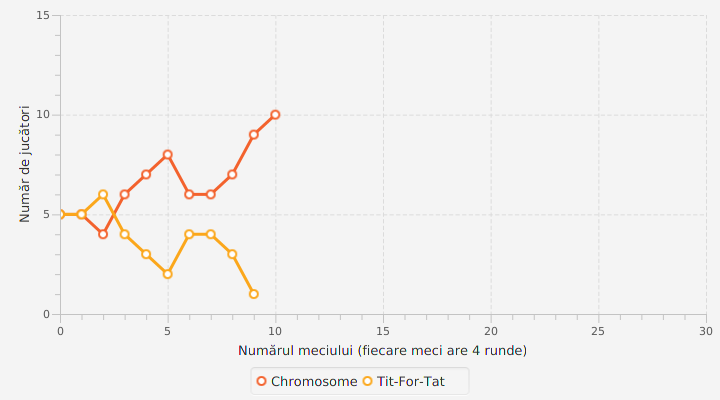
\includegraphics[	
		width=16cm,
		height=7.5cm,
		keepaspectratio
	]{imagini/experiment_5_epoch_1529329866051/chart_from_epoch_1530552284074.png}
	\caption{\textit{Cromozomii câștigă turneul cu eliminare în cadrul unui număr mic de runde, câte 4 runde la fiecare meci al turneului cu eliminare.}}
\end{figure}

Atunci când doi indivizi ce urmează startegia \textbf{Tit-For-Tat} concurează într-un meci, vor coopera la fiecare rundă iar cooperarea mutuală este cea mai bine răsplătită, oferind un punctaj pe măsură. Din acest motiv, la un turneu cu eliminare unde numărul de runde este mai mare (mai mare de 5 runde la fiecare meci), va depăși strategiile care trădează în majoritatea rundelor. 

\begin{figure}[H]
	\centering
	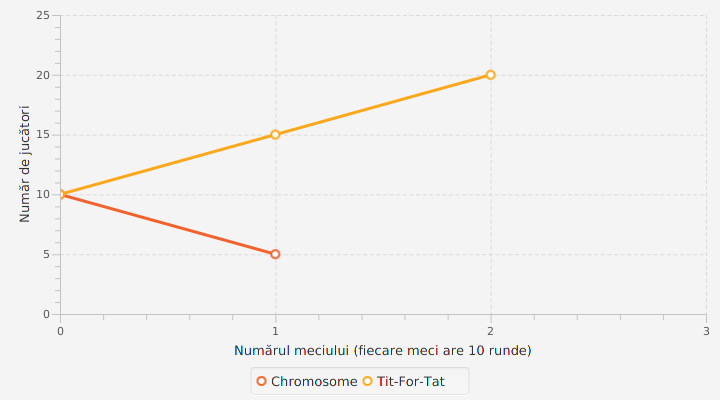
\includegraphics[	
		width=16cm,
		height=7.5cm,
		keepaspectratio
	]{imagini/experiment_5_epoch_1529329866051/chart_from_epoch_1529413879261.png}
	\caption{\textit{Strategia \textbf{Tit-For-Tat} câștigă când numărul de runde este 10.}}
\end{figure}

\begin{center}
	\underline{\textit{Experimentul numărul 6}}
\end{center}

\textit{Configurația algoritmului genetic și cea a turneului cu eliminare este trecută în \textbf{Anexa numărul 6}}.\\

Mai există o altă variantă pentru a învinge o populație dată de copii după \textbf{Tit-For-Tat}. 
 
Am făcut un experiment în care populația de antrenament este dată de un individ cu strategia \textbf{Tit-For-Tat}. Acest lucru a făcut ca strategia oferită de algoritmul genetic să imite strategia \textbf{Tit-For-Tat}. În aceste cazuri, cromozomii și copiile după \textbf{Tit-For-Tat} vor avea același scor și, la rundele eliminatorii, se vor elimina (și apoi duplica) la întâmplare câteva strategii dintre cele două tipuri. Sunt șanse egale de câştig între cele două tipuri de strategii.

\begin{figure}[H]
	\centering
	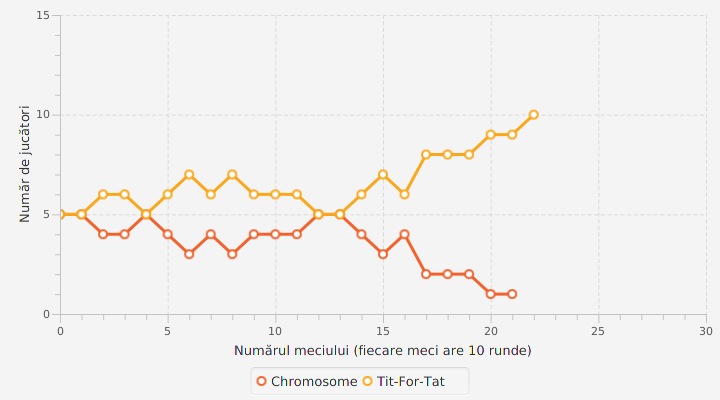
\includegraphics[	
		width=16cm,
		height=7.5cm,
		keepaspectratio
	]{imagini/experiment_6_epoch_1529327580314/chart_from_epoch_1529416356254.png}
	\caption{\textit{Populația ce folosește strategia \textbf{Tit-For-Tat} câștigă.}}
\end{figure}

\begin{figure}[H]
	\centering
	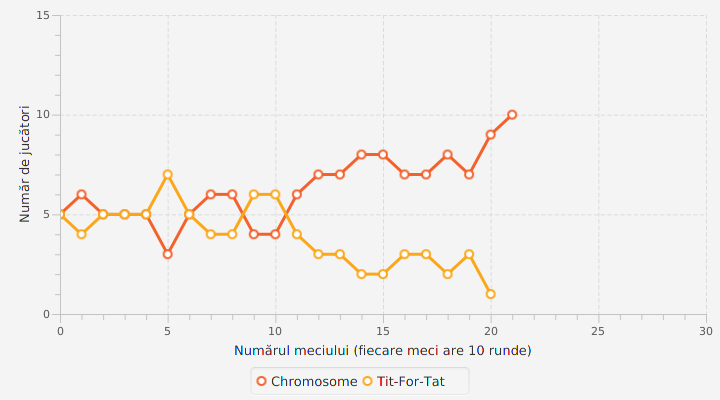
\includegraphics[	
		width=16cm,
		height=7.5cm,
		keepaspectratio
	]{imagini/experiment_6_epoch_1529327580314/chart_from_epoch_1529416343328.png}
	\caption{\textit{Cromozomii câștigă.}}
\end{figure} 













































































































































































































% Bibliografie 

\begin{thebibliography}{99}

\bibitem{introduction_by_melanie_mitchell}
Melanie Mitchell.
\textit{An introduction to Genetic Algorithms}

\bibitem{article_by_melanie_mitchell} 
Melanie Mitchell. 
\textit{Genetic Algorithms: An Overview}. 1995

\bibitem{adaptation_in_natural_and_artificial_systems}
John Holland. 
\textit{Adaptation in Natural and Artificial Systems}. 1975/1992

\bibitem{curs_prof_gabriel_oltean_cluj}
Prof. dr. ing. Gabriel Oltean.
\textit{Cursul de Tehnici de inteligenţă computaţională în electronică}
. Universitatea Tehnica din Cluj-Napoca
\\\texttt{http://www.bel.utcluj.ro/rom/dce/goltean/tice/10\_AlgoritmiGenetici.pdf}
\\\texttt{http://www.bel.utcluj.ro/dce/didactic/tice/tice.htm}

\bibitem{javaFX} 
Biblioteca JavaFX:\\
\texttt{http://www.oracle.com/technetwork/java/javase/}\\
\texttt{overview/javafx-overview-2158620.html}

\bibitem{slf4j} 
Biblioteca SLF4J:\\
\texttt{https://www.slf4j.org/}

\bibitem{json-simple} 
Biblioteca json-simple:\\
\texttt{https://cliftonlabs.github.io/json-simple/}

\bibitem{schita_algoritm_genetic}
Schema algoritm genetic:
\\\texttt{goo.gl/YLUE4i}\\
Din lucrarea: Bo Xu, Hongfei Lin, Kavishwar B Wagholikar, Zhihao Yang, Hongfang Liu. \textit{Identifying protein complexes with fuzzy machine learning model}
\\\texttt{https://goo.gl/SrAHpD} 

\bibitem{curs_daniela_zaharie} 
Prof. dr. Daniela Zaharie:\\
\textit{Cursul de Calcul neuronal și calcul evolutiv}
. Facultatea de Matematică si Informatică, Universitatea de Vest din Timişoara
\\\texttt{goo.gl/hQxKeh}

\end{thebibliography}	

\end{document}